\section{}
\textit{Explosions send blast waves from the centre, which consist of an initial positive pressure wave front followed by a phase of negative pressure which pulls objects back towards the detonation centre. For this question, consider the positive pressure phase of a blast wave as shown below. Typically, the blast wave last 100 ms, and reaches a max pressure (gage) of around 70 kPa.}
\begin{figure}[H]
    \centering
    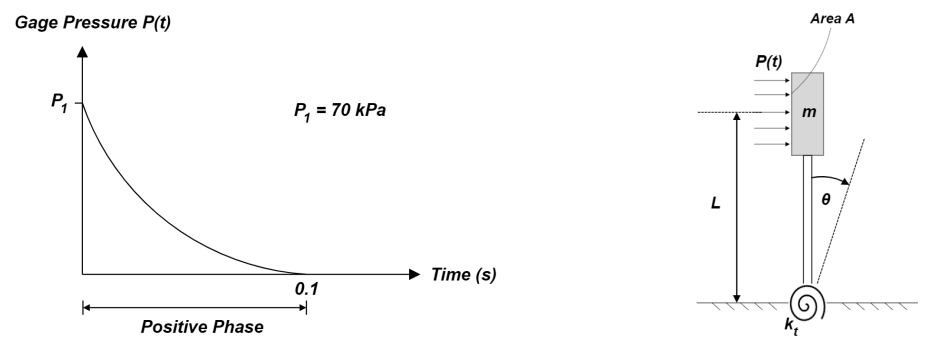
\includegraphics[width=0.7\linewidth]{Questions/Figures/Q3 Problem Diagram.png}
\end{figure}
\textit{A nearby road sign (shown above on the right), is approximated by a massless rod supporting a uniform thin disk (viewed from the side) of mass $m$, radius $r$, and frontal area $A$. The centre of the disk is at a height $L = 2r$ from the ground, and the ground connection is modelled as a torsional spring $k$. Assume that the pressure-time relation during the positive phase is approximated as:}
\begin{align*}
    P(t) = \frac{P_1}{4} \left(e^{-at} + 3e^{-bt} - 6t\right), \quad 0 \leq t \leq 0.1 \text{ s}
\end{align*}
\textit{The moment of inertia of a thin disk about its central diameter is $J = \frac{1}{4} m r^2$.}
\begin{enumerate}[label=(\alph*)]
    \item \textit{For the relation described above, determine the equation of motion for the sign during the positive phase in terms of $m$, $L$, $P(t)$, $k$, and $A$. Use as your coordinate $t$, $A g \theta$.}
    \item \textit{If the sign is initially at rest and $a = 10$, $b = 25$, $m = 1.5$ kg, $r = 0.25$ m, and $k = 1 \times 10^3$ Nm, calculate the response of the sign during the positive phase of the blast wave. You can neglect gravity in this case ($k$ dominates the effective stiffness).}
\end{enumerate}

\subsection*{Solution}
\subsection{}
The freebody diagram is as follows,
\begin{figure}[H]
    \centering
    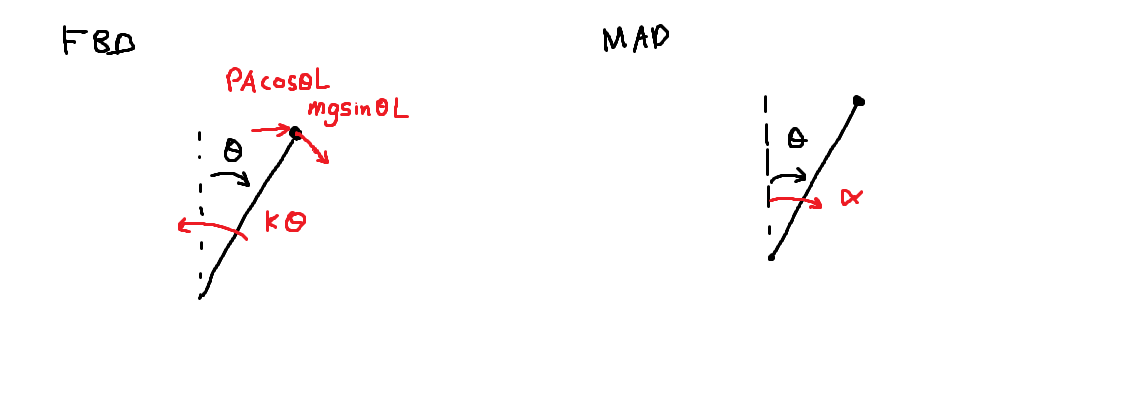
\includegraphics[width=0.7\linewidth]{Questions/Figures/Q3 FBD and MAD.png}
    \caption{Freebody Diagram and Mass Acceleration Diagram}
\end{figure}
The moment of inertia is given about the central diameter. Since the sign is experiencing pure rotation about the pin, it is convenient to move the moment of inertia to the IC,
\begin{align*}
    J_{\text{IC}} &= J_G + m L^2 \\
    &= \frac{1}{4} m r^2 + m L^2 \\
    &= \frac{1}{4} m \left(\frac{L}{2}\right)^2 + m L^2 \\
    &= \frac{1}{16} m L^2 + m L^2 \\
    &= \frac{17}{16} m L^2
\end{align*}
The area of the sign is 
\begin{align*}
    A &= \pi r^2 \\
    &= \pi \left(\frac{L}{2}\right)^2 \\
    &= \frac{\pi L^2}{4}
\end{align*}
The equation of motion is given by,
\begin{align*}
    \circlearrowright \sum M_{\text{IC}} &= J_{\text{IC}} \ddot{\theta} \\
    &= -k_t \theta + P A L \cos\theta + mgL \sin\theta 
\end{align*}
Rearranging,
\begin{empheq}[box=\fbox]{align*}
    \frac{17}{16} m L^2 \ddot{\theta} + k_t \theta - mgL \sin\theta = \frac{\pi P L^3}{4} \cos\theta
\end{empheq}
Assuming small angle approximation, $\sin\theta \approx \theta$ and $\cos\theta \approx 1$,
\begin{empheq}[box=\fbox]{align*}
    \underbrace{\left[\frac{17}{16} m L^2\right]}_{m_{\text{eff}}} \ddot{\theta} + \underbrace{\left[k_t - mgL\right]}_{k_{\text{eff}}} \theta = \underbrace{\frac{\pi P(t) L^3}{4}}_{F(t)} 
\end{empheq}

\subsection{}
Let us rewrite the forcing term, $F(t)$, in a more convenient form,
\begin{align*}
    F(t) &= \frac{\pi L^3}{4}\cdot \frac{P_1}{4} \left(e^{-at} + 3e^{-bt} - 6t \right) \\
    &= \frac{\pi P_1 L^3}{16} \left(e^{-at} + 3e^{-bt} - 6t \right) \\
    & = \underbrace{\frac{\pi P_1 L^3}{16}}_{F_1} e^{-at} + \underbrace{\frac{3\pi P_1 L^3}{16}}_{F_2} e^{-bt} + \underbrace{\frac{-3\pi P_1 L^3}{8}}_{\beta} t
\end{align*}
Neglecting gravity, the differential is now
\begin{align*}
    \underbrace{\left[\frac{17}{16} m L^2\right]}_{m_{\text{eff}}} \ddot{\theta} + \underbrace{\left[k_t\right]}_{k_{\text{eff}}} \theta = \underbrace{\frac{\pi P_1 L^3}{16}}_{F_1} e^{-at} + \underbrace{\frac{3\pi P_1 L^3}{16}}_{F_2} e^{-bt} + \underbrace{\frac{-3\pi P_1 L^3}{8}}_{\beta} t
\end{align*}
Substituting numbers,
\begin{align*}
    m_{\text{eff}} &= \frac{17}{16} \times 1.5 \times (2 \times 0.25)^2 = 0.3984375 \\
    k_{\text{eff}} &= 1 \times 10^3 \\
    p &= \sqrt{\frac{k_{\text{eff}}}{m_{\text{eff}}}} = \sqrt{\frac{1000}{0.3984375}} = 50.1 \\
    F_1 &= \frac{\pi \times 70 \times 10^3 \times (2 \times 0.25)^3}{16} = 1718.0585 \\
    F_2 &= \frac{3\pi \times 70 \times 10^3 \times (2 \times 0.25)^3}{16} = 5154.1754 \\
    \beta &= \frac{-3\pi \times 70 \times 10^3 \times (2 \times 0.25)^3}{8} = -10308.3509 
\end{align*}
The homogeneous solution is given by,
\begin{align*}
    \theta_H(t) &= C_1 \sin p t + C_2 \cos p t \\
    &= C_1 \sin (50.1 t) + C_2 \cos (50.1 t)
\end{align*}
The particular solution due to $F_1 e^{-at}$ is given by Eq. (7.7) from the textbook,
\begin{align*}
    \theta_{p1}(t) &= \frac{F_1}{m_{\text{eff}} a^2 + k_{\text{eff}}} e^{-at} \\
    &= \frac{1718.0585}{0.3984375 \times 100 + 1000} e^{-10t} \\
    &= 1.652 e^{-10t}
\end{align*}
The particular solution due to $F_2 e^{-bt}$ is given by Eq. (7.7) from the textbook,
\begin{align*}
    \theta_{p2}(t) &= \frac{F_2}{m_{\text{eff}} b^2 + k_{\text{eff}}} e^{-bt} \\
    &= \frac{5154.1754}{0.3984375 \times 625 + 1000} e^{-25t} \\
    &= 4.1266 e^{-25t}
\end{align*}
The particular solution due to $\beta t$ is given by Eq. (7.5) from the textbook,
\begin{align*}
    \theta_{p3}(t) &= \frac{\beta}{k} t \\
    &= \frac{-10308.3509}{1000} t \\
    &= -10.3084 t
\end{align*}
The total response is the sum of the homogeneous and particular solutions,
\begin{align*}
    \theta(t) &= \theta_{H}(t) + \theta_{p1}(t) + \theta_{p2}(t) + \theta_{p3}(t) \\
    &= C_1 \sin (50.1 t) + C_2 \cos (50.1) t + 1.652 e^{-10t} + 4.1266 e^{-25t} - 10.3084 t
\end{align*}
Applying the initial conditions,
\begin{align*}
    \theta(0) &= 0 \\
    \dot{\theta}(0) &= 0
\end{align*}
First, applying the initial condition $\theta(0) = 0$,
\begin{align*}
    \theta_{H}(0) &= C_2 \\
    \theta_{p1}(0) &= 1.652 \\
    \theta_{p2}(0) &= 4.1266 \\
    \theta_{p3}(0) &= 0 \\
\end{align*}
Substituting the values into the total response,
\begin{align*}
    \theta(0) &= C_2 + 1.652 + 4.1266 = 0 \\
    C_2 &= -5.7786
\end{align*}
Next, applying the initial condition $\dot{\theta}(0) = 0$,
\begin{align*}
    \dot{\theta}_{H}(0) &= 50.1 C_1 \\
    \dot{\theta}_{p1}(0) &= -10 \times 1.652 = -16.52 \\
    \dot{\theta}_{p2}(0) &= -25 \times 4.1266 = -103.165 \\
    \dot{\theta}_{p3}(0) &= -10.3084 \\
\end{align*}
Substituting the values into the total response,
\begin{align*}
    \dot{\theta}(0) &= 50.1 C_1 - 16.52 - 103.165 - 10.3084 = 0 \\
    C_1 &= 2.59
\end{align*}
The response is then,
\begin{empheq}[box=\fbox]{align*}
    \theta(t) &= 2.59 \sin (50.1 t) - 5.7786 \cos (50.1 t) + 1.652 e^{-10t} + 4.1266 e^{-25t} - 10.3084 t
\end{empheq}
